\documentclass[11pt,a4paper]{article}
\usepackage[a4paper,top=14mm,bottom=14mm,left=15mm,right=15mm]{geometry}
\usepackage[T1]{fontenc}
\usepackage{amsmath}
\usepackage{amssymb}
\usepackage{array}
\usepackage{multicol}
\usepackage{tikz}
\usetikzlibrary{arrows.meta,decorations.pathreplacing}

% ================================================================
% Fractions, decimals and percentages: revision questions.
%
% Two pages of questions, in black and white, with a heading for each
% topic on the Maths Revision topic list in the same order. Each topic
% has a few short questions that start easy, with a diagram only where
% a question uses one, and the sheet ends with some problem solving.
% There are no key facts or worked examples on the sheet: the methods
% are in the worked solutions and the revision guide. Questions are
% numbered through the sheet so that the answer key and the worked
% solutions can refer to them.
% ================================================================

\pagestyle{empty}
\setlength{\parindent}{0pt}
\setlength{\parskip}{2pt}
\setlength{\columnsep}{9mm}

% A topic from the revision list.
\newcommand{\topic}[1]{\par\addvspace{9pt}{\bfseries #1}\par\nobreak\vspace{2pt}}

% Questions are numbered through the whole sheet.
\newcounter{qn}
\newcommand{\q}{\par\addvspace{5pt}\stepcounter{qn}\hangindent=1.6em\hangafter=1\noindent
  \makebox[1.6em][l]{\textbf{\theqn}}}

% \fracbars{<bars>}{<parts in each bar>}{<parts shaded>}{<bars in a row>}{<part width>}
\newcommand{\fracbars}[5]{%
  \begin{tikzpicture}[x=#5,y=4mm]
    \foreach \b in {1,...,#1}{%
      \pgfmathtruncatemacro{\fcr}{(\b-1)/#4}%
      \pgfmathtruncatemacro{\fcc}{mod(\b-1,#4)}%
      \foreach \p in {1,...,#2}{%
        \pgfmathtruncatemacro{\fck}{(\b-1)*#2+\p}%
        \pgfmathsetmacro{\fcx}{\fcc*(#2+0.8)+\p-1}%
        \pgfmathsetmacro{\fcy}{-\fcr*1.6}%
        \ifnum\fck>#3\relax
          \draw (\fcx,\fcy) rectangle ++(1,1);
        \else
          \draw[fill=black!15] (\fcx,\fcy) rectangle ++(1,1);
        \fi}}
  \end{tikzpicture}}

% \hundredgrid{<squares shaded>}{<square size>}: shaded row by row.
\newcommand{\hundredgrid}[2]{%
  \begin{tikzpicture}[x=#2,y=#2]
    \foreach \i in {0,...,99}{%
      \pgfmathtruncatemacro{\r}{\i/10}%
      \pgfmathtruncatemacro{\c}{mod(\i,10)}%
      \ifnum\i<#1\relax \fill[black!15] (\c,-\r) rectangle ++(1,1);\fi}
    \draw[step=1] (0,-9) grid (10,1);
  \end{tikzpicture}}

\begin{document}
% Ragged right, without \raggedright, which would make \\ end the
% paragraph and lose the hanging indent of a question's later lines.
\setlength{\rightskip}{0pt plus 4em}

{\Large\bfseries Fractions, decimals and percentages}\hfill{\large Revision questions}
\par\vspace{2pt}\hrule\vspace{4pt}

\begin{multicols}{2}

% ----------------------------------------------------------------
\topic{Simplifying fractions}
\q What fraction of the bar is shaded? Give your answer in its simplest form.\\[4pt]
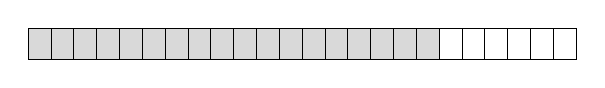
\begin{tikzpicture}[x=2.9mm,y=4mm]
  \fill[black!15] (0,0) rectangle (18,1);
  \foreach \i in {0,...,23}{\draw (\i,0) rectangle ++(1,1);}
\end{tikzpicture}
\q Simplify\quad (a) $\dfrac{12}{16}$\qquad (b) $\dfrac{30}{45}$\qquad (c) $\dfrac{84}{120}$

% ----------------------------------------------------------------
\topic{Ordering fractions}
\q Write in order, smallest first.\\[2pt]
(a) $\dfrac34,\ \dfrac58,\ \dfrac7{12}$\qquad (b) $\dfrac45,\ \dfrac7{10},\ \dfrac34,\ \dfrac{13}{20}$
\q Ella eats $\frac38$ of a pizza. Sam eats $\frac25$ of an identical pizza. Who eats more?

% ----------------------------------------------------------------
\topic{Mixed numbers and improper fractions}
\q Write the shaded amount as\\
(a) a mixed number\qquad (b) an improper fraction.\\[4pt]
\fracbars{3}{4}{11}{3}{4.4mm}
\q (a) Write $5\frac23$ as an improper fraction.\\
(b) Write $\frac{31}6$ as a mixed number.

% ----------------------------------------------------------------
\topic{Adding and subtracting fractions}
\q (a) $\dfrac13+\dfrac15$\qquad (b) $\dfrac34-\dfrac27$\qquad (c) $\dfrac56+\dfrac38$
\q Jack spends $\frac14$ of his money on a game and $\frac25$ of it on clothes. What fraction of his money is left?

% ----------------------------------------------------------------
\topic{One number as a percentage of another}
\q Write as a percentage.\\
(a) 12 out of 50\qquad (b) 27 out of 60\\
(c) 35\,cm out of 2\,m
\q Priya scores 34 out of 40 in a test. Leo scores 41 out of 50. Who did better?

% ----------------------------------------------------------------
\topic{Percentages without a calculator}
\q Find\quad (a) 10\% of 470\qquad (b) 50\% of 86\\
(c) 1\% of 650\qquad (d) 15\% of 360
\q A £45 jacket is reduced by 20\% in a sale. What is the sale price?

% ----------------------------------------------------------------
\columnbreak
\topic{Converting between fractions, decimals and percentages}
\q Write the shaded part of the grid as a fraction in its simplest form, as a decimal and as a percentage.\\[4pt]
\hundredgrid{36}{2.2mm}
\q Copy and complete the table.\\[4pt]
{\renewcommand{\arraystretch}{1.5}%
\begin{tabular}{|c|c|c|}\hline
\ Fraction\ & \ Decimal\ & Percentage\\\hline
$\frac35$ & & \\\hline
 & 0.45 & \\\hline
 & & 4\%\\\hline
\end{tabular}}

% ----------------------------------------------------------------
\topic{Ordering fractions, decimals and percentages}
\q Write in order, smallest first.\\
(a) 0.4,\ \ $\frac38$,\ \ 41\%\qquad (b) $\frac13$,\ \ 0.3,\ \ 33\%
\q Shop A takes $\frac13$ off its prices. Shop B takes 30\% off. Shop C takes 0.35 of the price off. Which shop gives the biggest discount?

% ----------------------------------------------------------------
\topic{Fractions of amounts}
\q Use the bar model to find $\frac35$ of 60.\\[4pt]
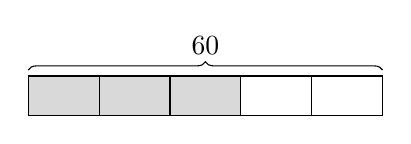
\begin{tikzpicture}[x=9mm,y=5mm]
  \fill[black!15] (0,0) rectangle (3,1);
  \foreach \i in {0,...,4}{\draw (\i,0) rectangle ++(1,1);}
  \draw[decorate,decoration={brace,amplitude=3pt}] (0,1.15) -- (5,1.15) node[midway,above=2pt] {60};
\end{tikzpicture}
\q (a) Without a calculator, find $\frac38$ of 64.\\
(b) With a calculator, find $\frac79$ of 504.
\q A school has 840 pupils. $\frac37$ of them have school dinners. How many pupils do not have school dinners?

% ----------------------------------------------------------------
\topic{Percentages of amounts}
\q Without a calculator, find\\
(a) 35\% of 140\qquad (b) 12.5\% of 64
\q With a calculator, find\\
(a) 23\% of 85\qquad (b) 4.5\% of £2400

% ----------------------------------------------------------------
\topic{Percentage change}
\q Find the percentage change.\\
(a) 50\,kg to 62\,kg\qquad (b) £80 to £68
\q A car bought for £12\,000 is sold two years later for £9000. Find the percentage decrease.

\end{multicols}

\newpage

\begin{multicols}{2}

% ----------------------------------------------------------------
\topic{Simple interest}
\q £500 is invested at 2\% simple interest per year. Copy and complete the table.\\[4pt]
{\renewcommand{\arraystretch}{1.5}%
\begin{tabular}{|l|c|c|c|c|c|}\hline
Year & 0 & 1 & 2 & 3 & 4\\\hline
Balance (£) & 500 & \hspace{6mm} & \hspace{6mm} & \hspace{6mm} & \hspace{6mm}\\\hline
\end{tabular}}
\q Amy invests £800 at 5\% simple interest per year. After how many years will she have £1000?

% ----------------------------------------------------------------
\topic{Calculating with mixed numbers and negatives}
\q (a) $1\dfrac23+2\dfrac14$\qquad (b) $4\dfrac15-1\dfrac12$\qquad (c) $1\dfrac12\times2\dfrac23$
\q (a) $3\dfrac34\div1\dfrac14$\qquad (b) $-\dfrac23\times\dfrac9{10}$\\[4pt]
(c) $-1\dfrac14\div\left(-\dfrac58\right)$

% ----------------------------------------------------------------
\topic{Word problems with mixed numbers}
\q A plank is $5\frac14$\,m long. A piece $2\frac23$\,m long is cut off. How long is the piece that is left?\\[4pt]
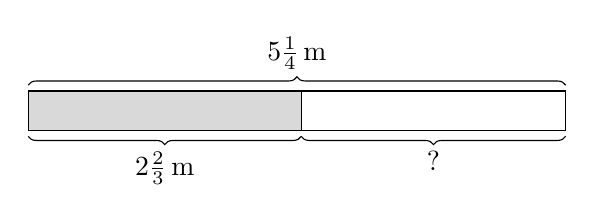
\begin{tikzpicture}[x=13mm,y=5mm]
  \fill[black!15] (0,0) rectangle (2.667,1);
  \draw (0,0) rectangle (5.25,1) (2.667,0) -- (2.667,1);
  \draw[decorate,decoration={brace,amplitude=3pt}] (0,1.15) -- (5.25,1.15) node[midway,above=2pt] {$5\frac14$\,m};
  \draw[decorate,decoration={brace,amplitude=3pt,mirror}] (0,-0.15) -- (2.667,-0.15) node[midway,below=2pt] {$2\frac23$\,m};
  \draw[decorate,decoration={brace,amplitude=3pt,mirror}] (2.667,-0.15) -- (5.25,-0.15) node[midway,below=2pt] {?};
\end{tikzpicture}
\q How many $\frac13$ litre glasses can be completely filled from a jug holding $2\frac34$ litres?
\q A rectangular garden is $6\frac12$\,m long and $3\frac13$\,m wide. Find its area.

% ----------------------------------------------------------------
\topic{Recurring decimals to fractions}
\q Copy and complete to write $0.\dot4$ as a fraction.\\[3pt]
\begin{tabular}{@{}r@{\;=\;}l@{}}
  Let $n$ & $0.444\ldots$\\[3pt]
  $10n$ & \rule{18mm}{0.4pt}\\[3pt]
  subtract:\ \ \rule{8mm}{0.4pt}\,$n$ & \rule{18mm}{0.4pt}\\[3pt]
  $n$ & \rule{18mm}{0.4pt}
\end{tabular}
\q Write as fractions in their simplest form.\\
(a) $0.\dot3\dot6$\qquad (b) $0.8\dot3$

% ----------------------------------------------------------------
\topic{Percentage increase and decrease with multipliers}
\q Write down the multiplier for\\
(a) an increase of 8\%\qquad (b) a decrease of 30\%\\
(c) an increase of 2.5\%
\q (a) Increase £64 by 35\%.\\
(b) Decrease 1250 by 12\%.

% ----------------------------------------------------------------
\topic{Finding the original amount}
\q In a sale, everything is 30\% off. A coat costs £56 in the sale. What was the original price?\\[4pt]
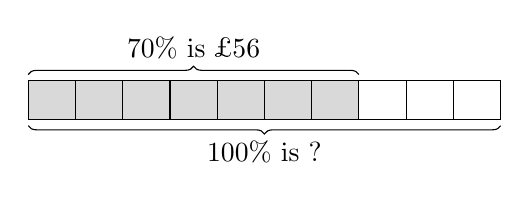
\begin{tikzpicture}[x=6mm,y=5mm]
  \fill[black!15] (0,0) rectangle (7,1);
  \foreach \i in {0,...,9}{\draw (\i,0) rectangle ++(1,1);}
  \draw[decorate,decoration={brace,amplitude=3pt}] (0,1.15) -- (7,1.15) node[midway,above=2pt] {70\% is £56};
  \draw[decorate,decoration={brace,amplitude=3pt,mirror}] (0,-0.15) -- (10,-0.15) node[midway,below=2pt] {100\% is ?};
\end{tikzpicture}
\q After a 10\% increase, a bill is £77. What was the bill before the increase?
\q A price including 20\% VAT is £54. What was the price before VAT was added?

% ----------------------------------------------------------------
\topic{Problem solving}
\q A £90 coat is on sale in two shops. Shop A takes $\frac13$ off. Shop B takes 30\% off, then a further 5\% off the sale price. Which shop is cheaper, and by how much?
\q Kim says, ``After 30\% off, a bike costs £280, so the original price was $280\times1.3=$ £364.'' Explain Kim's mistake, and find the correct original price.
\q Write down three different fractions between $\frac35$ and $\frac7{10}$. Show how you know that each one is in this range.

\end{multicols}

\end{document}
